% Chapter 1

\chapter{Introduction}

\label{intro} 

\graphicspath{{Figures/Introduction}}

Static typing is a typing discipline where types of expressions are checked at compile time. In practice, statically type programming languages offer many advantages:

It allows early error detection, enhances code readability, and promotes maintainability, especially in large collaborative projects. The explicit type information often improves tooling and IDE (interactive development environment) support. Additionally, static typing enhances the library documentation by providing clear contracts between library authors and uses.

Similarly, functional language is a programming language category where functional programming principles are enforced. These include immutable values and referential transparency. Like statical typing, functional language also helps avoid certain undesired behaviours of programs, such as misaligned pointers and race conditions, by removing or carefully separating the effectful computation from the pure one. In addition, functional programming promotes the idea of using functions as the fundamental building blocks of programming and developing abstractions by composing functions. For these reasons, functional programming languages are often taught to beginners. Lastly, functional language's strict immutability provides distinct advantages in concurrency and parallelism.

Combining the two disciplines, statically typed functional languages employ both static typing and functional paradigm. These languages, such as Haskell and ML, provide the strongest level of programming safety. It is often advertised that programs in these languages will be error-free if the source code passes the compiling stage, indicating that compilers are able to weed out many different classes of errors. With these safety properties, statically typed functional languages are often used as proof assistance and formal verifications where rigorous type-checking is paramount. Despite the safety benefits, these languages failed to gain significant popularity in mainstream programming. This lack of popularity is often attributed to higher barriers to entry, unfamiliarity, and unforgiving type errors.

Type errors are one of the most blamed factors for posing hard barriers to learning and using statically typed functional language. Programmers often find type errors hard to read and understand when high-level abstractions are in play such as monads, type classes, and polymorphic types. Besides, type errors often use unfamiliar languages with liberal uses of jargon. Most importantly, the type error locations and explanations provided by traditional compiler tools are often misleading or wrong. All these factors make debugging type errors notoriously difficult.

Programming tools and environments, built with modern graphical interfaces, play a very important role in learning and using the language. Historically, the infamous Object-Oriented language Smalltalk benefited greatly from its flexible and powerful IDE. Other examples include DrScheme for teaching and supporting the Lisp language. However, efforts to improve type errors with modern technology have been lacking. In fact, in most statically typed functional languages, our tooling hasn’t changed for the last few decades and still remains in text format displayed in the terminal interface. 

\begin{figure}[hbt]
  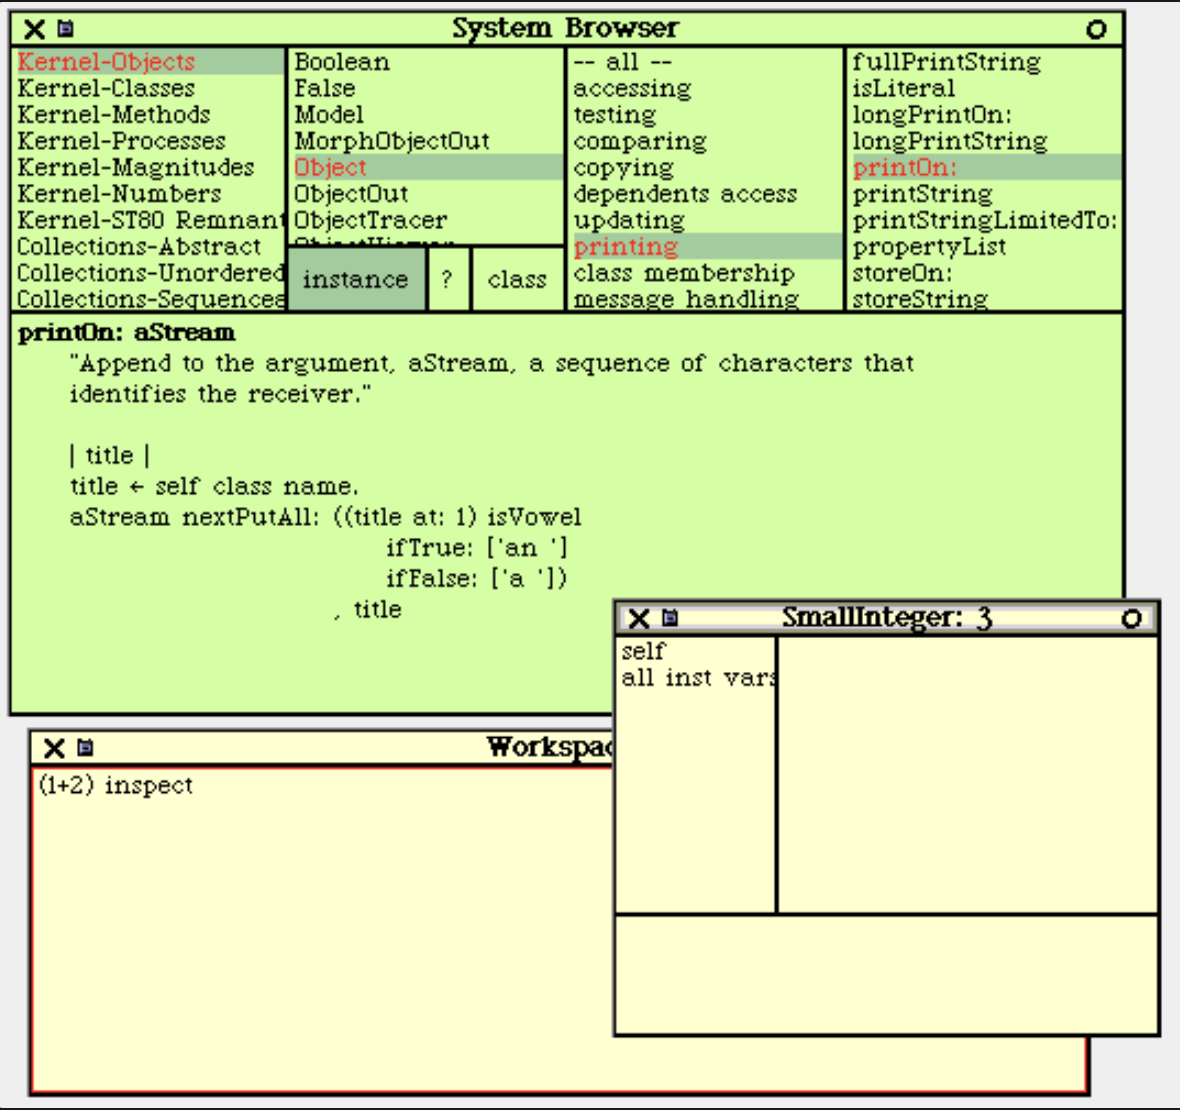
\includegraphics[width=\linewidth]{Smalltalk}
  \caption{
    An screenshot of smalltack IDE - Squeak
    }
\end{figure}


\begin{figure}[hbt]
  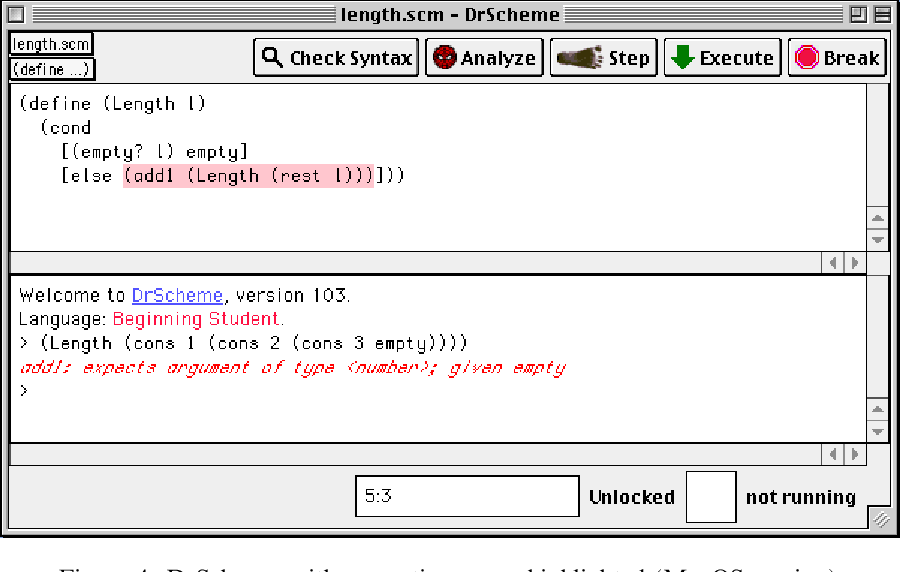
\includegraphics[width=\linewidth]{DrScheme}
  \caption{
    Dr Scheme, an Scheme IDE, highlighting a runtime error
    }
\end{figure}

My research is motivated by the inherent difficulties in debugging type errors and the dormant development of improving type errors with modern graphical interfaces and HCI techniques.

\section{Research Aim}

\subsection{Aim 1. To create rich type error data representations that can support interactive explanation, exploration and resolution of type errors.}

To date, there is no unified representation of type errors. But most contemporary compiler tools represent type error as the combination of three objects: a location where the failed type checking failed, an expected input, and the actually encountered input. [Give example here]

\subsubsection{Objective 1.1 Reflect that a type error may be caused by multiple locations.}

Traditional tools are limited to reporting a single location for the type error. This has been addressed by many researchers as an unhelpful limitation. Programmers are often unable to find resolution at the reported location and are forced to expand their search without guidance. We want to improve this by reporting accurate locations that are relevant to the type error.

\subsubsection{Objective 1.2 Reflect that there may be more than one explanation for a type error}

Erroneous programs can often be explained in multiple ways. When two pieces of evidence contradict each other, traditional tools choose the first one they encounter as the truth and the second one the culprit. When a contradiction consists of more than two pieces of evidence, traditional tools will generally ignore everything after the infeasibility is encountered. To improve this, first, we want to preserve the multiple explanations of type errors without picking sides. Second, we want to take into account all evidence.

\subsubsection{Objective 1.3 Reflect that there may be different causes of a type error.}

Type error does not end with a location in the source code. Programmers can still struggle to resolve a type error even after reaching the exact location of the culprits, failing to understand the logical explanation of the type error. Internally type error can be caused by mismatched types, unfulfilled type class constraints, or trying to construct infinite types. Externally, type error can be caused by typos, outdated type annotation, incomplete implementation, too few or too many arguments in a function application, etc.. Helping programmers find the cause or provide an accurate inference of what is the cause of the type error.

\subsection{Aim 2. Improve the understanding and resolving of type errors using modern programming environment and workflow}

To integrate rich type error data into a modern, visual programming environment and workflow that allows people to work more efficiently with strongly typed languages.


When humans are put in the middle, more information does not equal better comprehension. With enriched data representation, we want to deliver type errors to better support programmers’ comprehension and the chance for a successful resolution.

\subsubsection{Objective 2.1 Communicate the key concepts of type errors effectively using modern programming tools}

The concepts of type errors are traditionally displayed as text. These concepts include error locations, alternative explanations, causes and intermediate type signatures. We explore more intuitive techniques and media to communicate these concepts to better facilitate comprehension.

\subsubsection{Objective 2.2 Support programmers to interactively investigate and explore the type errors}

To avoid presenting overwhelming information, we explore different techniques of interactively exploring the type errors. These techniques include dividing the type error into small chunks that follow a linear line of reasoning, or bisecting the error one step at a time into smaller concepts.

\section{Contributions}

\subsection{Chameleon}

We contribute Chameleon, an interactive Haskell type error debugging tool. Internally, Chameleon computes all relevant locations that contribute to the type of error (1.2). Via a set of iteratively designed interface, Chameleon preserves the two alternatives of the type error and the supporting evidence for each (Objective 1.2).


We also contributed a series of studies of the effects of debugging with visual representation of types (Objective 2.1) and interactively explored type errors (Objective 2.2). We show that there is a difference between using traditional tools and enhanced type error debugging tools like Chameleon. And we show that this difference is more significant when debugging complex type errors.

\subsection{Goanna}
We contribute Goanna, a Haskell type error debugging tool. Like Chameleon, Goanna iterates relevant locations (Objective 1.1) that contribute to the type error and presents alternatives to the type error (Objective 1.2). Different from Chameleon, Goanna will exhaust all possible alternative explanations of the type error. Also, Goanna presents a type error by dividing it into a list of potential causes and their respective fixes (2.2). With Goanna, Haskell programmers can resolve type errors by exploring a list of potential error root causes. These causes are ordered using our heuristics so that the more likely causes are on top. We show that via our empirical evaluation that Goanna outperforms existing Haskell compilers when explaining the type error, with the slight disadvantage of an increased computation time.

\subsection{GeckoGraph}

We contribute GeckoGraph, a graphic notation for Haskell types. GeckoGraph describes the same information as a type signature does, but uses colours, shapes, and symbols to make certain structures easy to identify at a glance. GeckoGraph is designed to use visual elements to improve the understanding of type-level concepts (Objective 2.1). This includes type classes, parametric type variables, and high-rank types. When used to compare two types, GeckoGraph helps clarify differences visually. It makes errors like too few or too many arguments in applications, unmet type class constraints obvious.


We conducted a large-scale study on the effectiveness of using GeckoGraph to perform a series of Haskell tasks. We concluded that with GeckoGraph, programmers are able to succeed in harder tasks.


\section{Thesis outline}

The thesis begins with an overview of the challenges of type errors. We also outline the approaches that have been studied in the type theoretical direction and in the human-centred interaction direction. We then present our three projects, Chameleon, Goanna and GeckoGraph. Then, we propose a debugging system that combines the strengths of all the tools. We conclude the thesis with a discussion of the implications of our contribution to the understanding of type errors, tool designing, and programming language research. We then outline a few future directions of this work.

